\documentclass[a4paper,11pt,abstracton,titlepage]{scrartcl}
\usepackage[T1]{fontenc}
\usepackage[utf8]{inputenc}
\usepackage{lmodern}
\usepackage[ngerman]{babel}
\usepackage{eurosym}
\usepackage{textcomp}
\usepackage{graphicx}
\usepackage{geometry}
\usepackage{pdfpages}
\usepackage{wrapfig}

\usepackage{helvet}
\renewcommand{\familydefault}{\sfdefault}

% die Vorgaben der Prüfungsarbeit... etwas hässlich
\geometry{a4paper,left=25mm,right=25mm, top=3cm, bottom=3cm}
\parindent 0pt


\title{Clipboard-Manager\\Design und Programmierung}
\author{Simon Sperling\and Felix Nehrke\and Tobias Schult\and Wojciech
Rydzewski} % muss zum Schluss noch gefüllt werden
\date{29. Mai 2012}

\begin{document}

\maketitle

\tableofcontents
\thispagestyle{empty}
\newpage
% die Vorgaben der Prüfungsarbeit... etwas hässlich
\setlength{\parskip}{1em} 
\setcounter{page}{1}

\section{Einleitung}
In diesem Block haben wir uns eingehend mit dem Objektorientierten Design, sowie
der entsprechenden Programmierung beschäftigt.

\section{OOD Entwurf}
Als ersten Schritt zu unserer Implementierung haben wir unser Klassendiagramm
aus der Objektorientierten Analyse zu einem Objektorientierten Design
weiterentwickelt. Dabei haben wir vor Allem die technischen Gesichtspunkte
berücksichtigt um eine möglichst genaue Vorlage für die weitere Programmierung
zu erhalten.

Dieses Diagramm stellt die grundlegende Funktionalität dar, ohne das User
Interface oder andere zusätzliche Funktionen abzubilden. Das heißt, dass weder
die GUI, noch die Möglichkeit Einstellungen zu speichern oder zu laden darin
enthalten sind.

\begin{figure}[hb]
  \centering
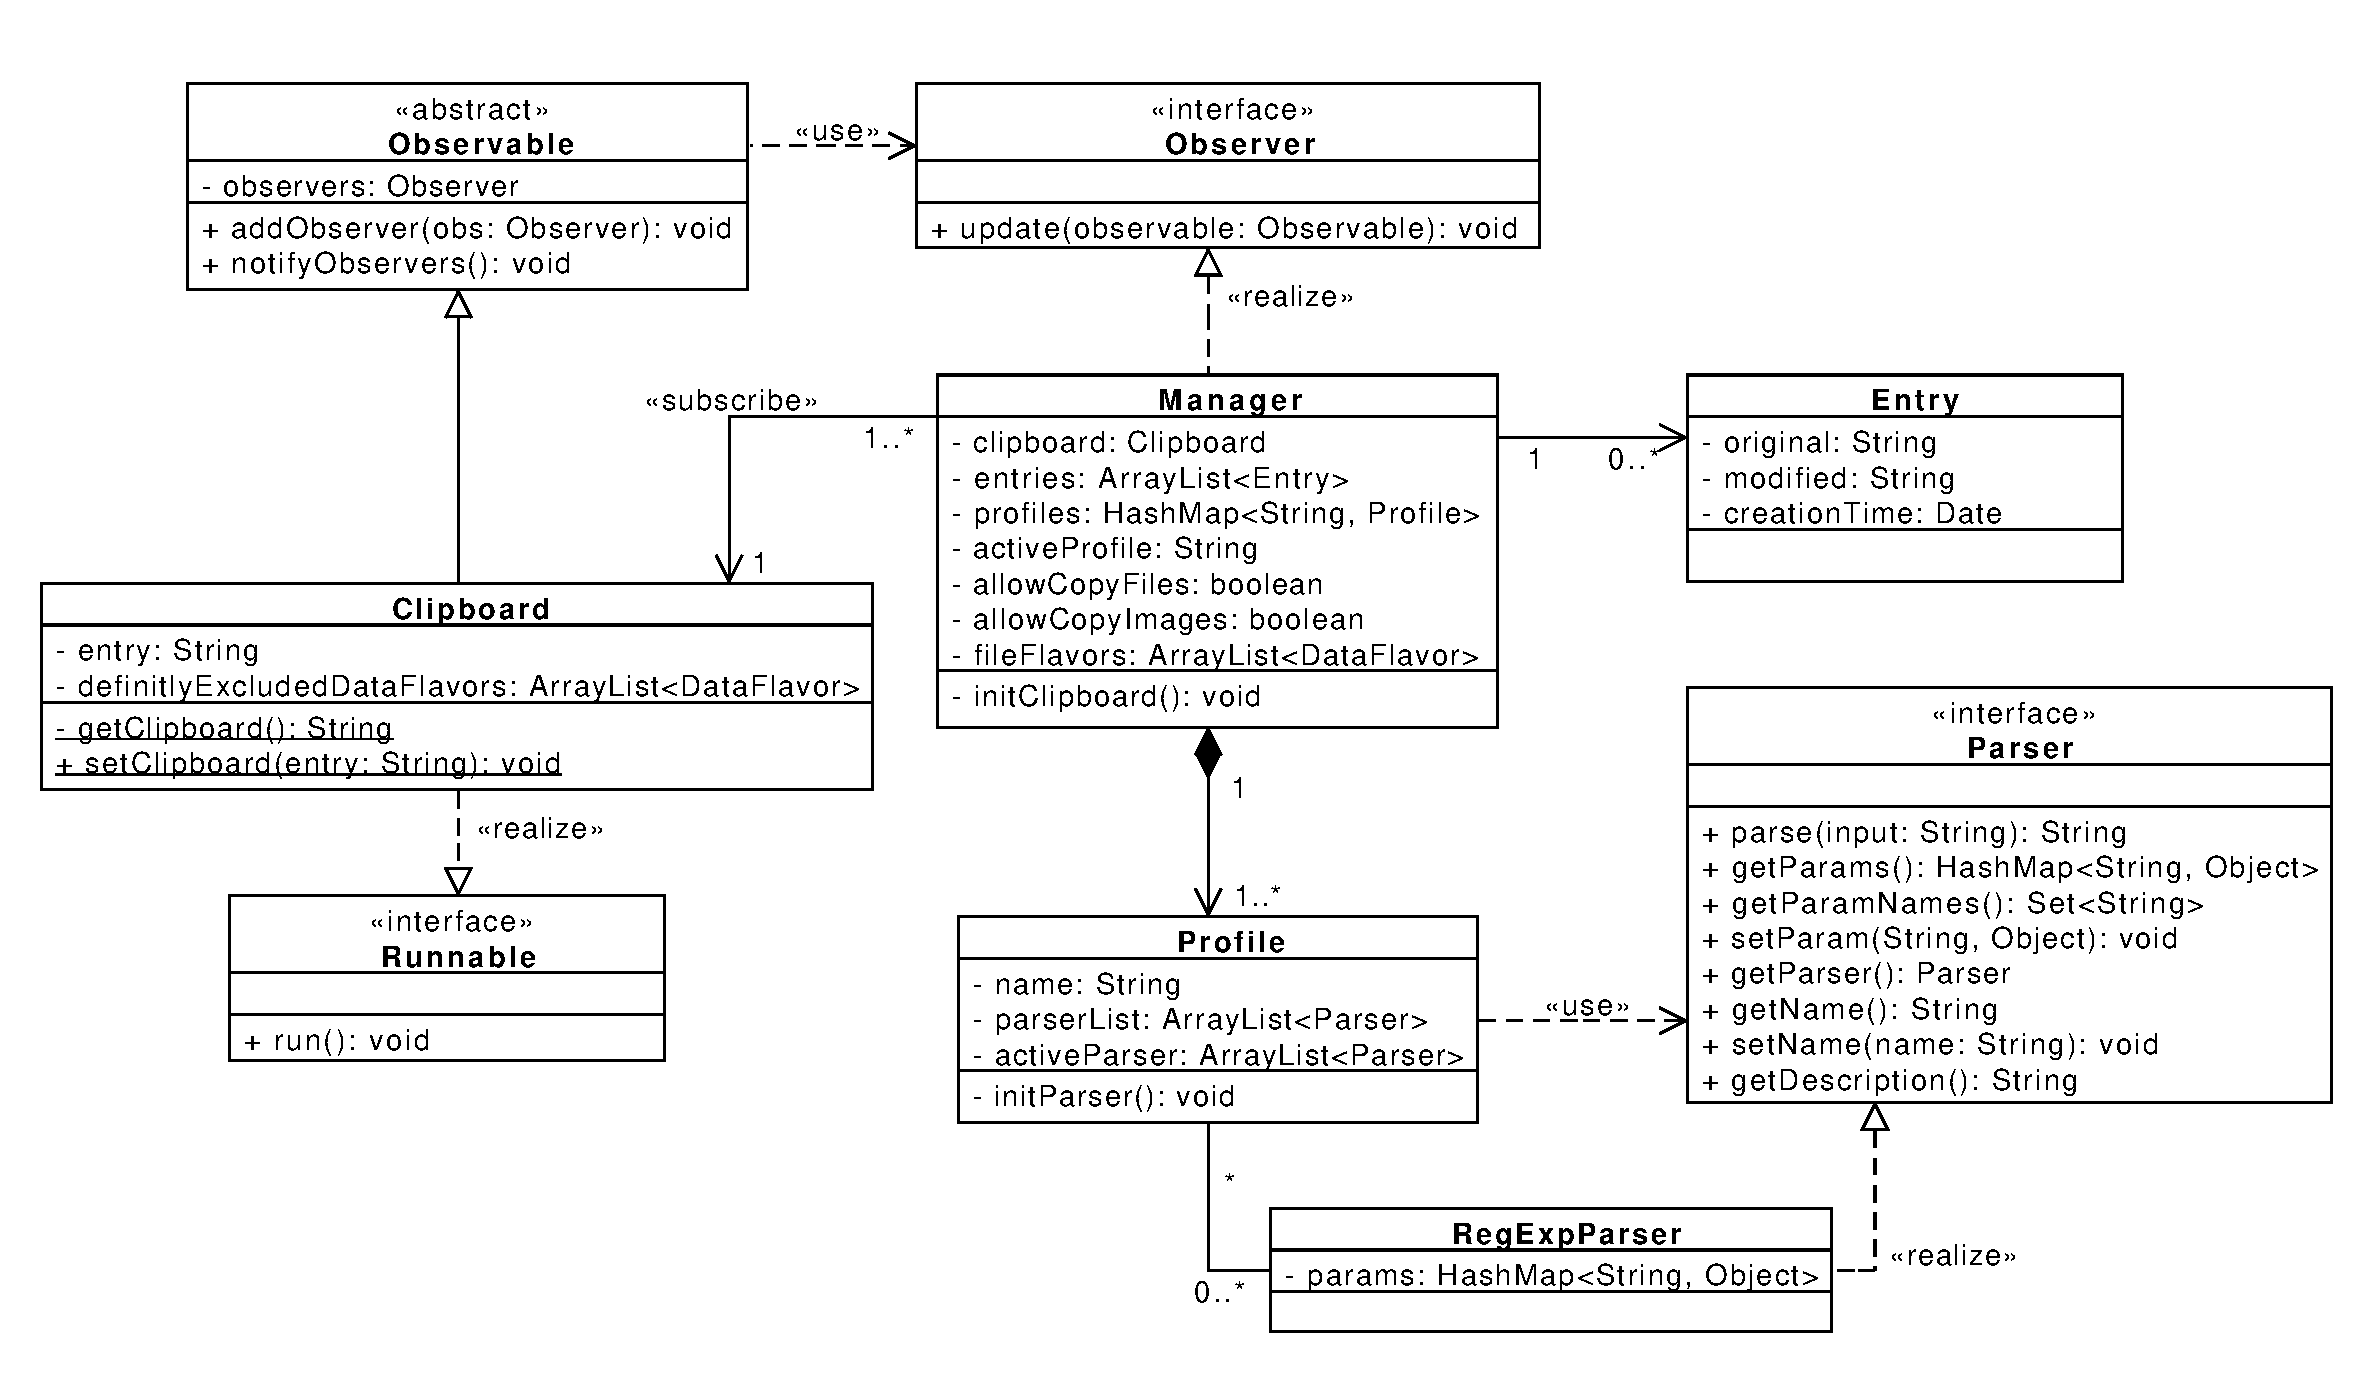
\includegraphics[width=\dimexpr\textwidth]{4-klassendiagramm-ood.pdf}
  \caption[OOD]%
  {Klassendiagramm des Objektorientierten Designs}
\end{figure}

Die Grafik zeigt alle wichtigen Klassen und Interfaces um das Programm
auszuführen. Den Kern stellt dabei das Managerobject dar, welches lose an das
Clipboard gebunden ist. Diese Verbindung wird über ein Observerpattern
realisiert, welches im weiteren Verlauf beschrieben wird. Dabei ist zu beachten,
dass der Manager vor allem selbst keine Funktionalität zur Verfügung stellt,
sondern lediglich die Verbindung zwischen den anderen Komponenten verwaltet.
Lediglich die Objekte der Entry-Klasse sind abhängig vom Manager. Diese
speichern den ursprünglichen Clipboardeintrag und den modifizierten Text,
welcher von den aktiven Parsern manipuliert wird.

Alle weitere Funktionalität hängt von den Profilen ab, welche verschiedene
Parser nutzen, um den Eintrag aus dem Clipboard zu parsen. Da die Parser in
einem Pluginsystem realisiert sind, ist in der Grafik lediglich ein Beispiel
abgebildet, welches eine RegExpParser zeigt. Grundsätzlich können aber
unterschiedlichste Methoden und Funktionen implementiert sein.

Um als Parser genutzt zu werden muss dieser als .jar Datei vorliegen und sich in
einem bestimmten Verzeichnis befinden. Außerdem muss er das Parser-interface
implementieren.


\section{Graphical User Interface -- GUI}
Die GUI dient bei unserem Programm zur Steuerung des Managers, der Profile und
der Parser. Die einzelnen Komponenten könnten auch durch ein anderes
User-Interface bedient werden, da sie selbständig Ihre Aufgaben erfüllen können.
Dementsprechend enthält die GUI keine systemrelevante Logik und wird lediglich
zur Steuerung genutzt.

\subsection{Hauptmenü}
Das Hauptmenü stellt einige zusätzliche Funktionen bereit, welche nicht
unbedingt nötig sind, aber das arbeiten mit dem Programm erheblich vereinfachen.
\subsubsection{Datei}
In diesem Menü können die Einstellungen geöffnet und gespeichert werden. Dabei
wird der Zustand des Programms (vorhandene Profile) in XML Format gespeichert /
ausgelesen. Der Vorteil an XML ist, dass wir eine Datei bekommen die man leicht
an mehrere Arbeitsplätze oder Mitarbeiter weiterreichen kann. Auch hiermit ist
es möglich eine Synchronisation zu ermöglichen, die allerdings einen Webservice
oder eine Datenbank erfordern würde.

\subsubsection{Einstellungen}
Da Java versucht jeglichen Inhalt aus der Zwischenablage auszulesen wird eine
kopierte Datei als Pfad interpretiert. Um den normalen Betrieb nicht zu
behindern lässt sich dieser Fall gesondert einstellen. 
\newpage
\subsection{Einträge / History}
\begin{wrapfigure}{r}{0.37\textwidth}
	\begin{center}
		\setlength{\fboxsep}{0pt}
		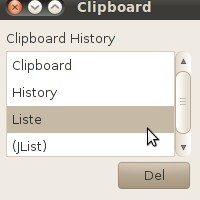
\includegraphics[width=\dimexpr0.33\textwidth-2pt\relax]{GUI_history.png}
	\end{center}
	\caption[GUI Einträge]
  {Ansicht der Einträge}
	\label{fig:Ressourcenbaum}
\end{wrapfigure}
Das Hauptfenster wurde in einem Raster umgesetzt. Das heißt, dass die Elemente
automatisch bei Veränderung der Fenstergröße an entsprechenden Stellen
ausgerichtet und teilweise vergrößert / verkleinert werden. Dies hat den
Vorteil, dass auch mehr Inhalt eines Eintrags angezeigt werden kann und eine
flexible Darstellung ermöglicht.

In der Liste, sieht der Nutzer seine bisher kopierten, nicht geparsten,
Einträge. Im untersten Teil des Fensters, sieht der Nutzer den letzten bzw. den
ausgewählten Eintrag. Um z.B. einen alten Eintrag wieder herzustellen, kann der
User in der Liste den gewünschten Inhalt auswählen und aus dem Textfeld wieder
in die Zwischenablage kopieren. Dies ist allerdings nur mit dem Tastaturkürzel
möglich. Hierbei sollte beachtet werden, dass ein neu kopierter Inhalt ebenfalls
durch aktive Parser verändert werden kann, für den Fall lassen sich die Parser
einfach über die Checkbox ausschalten.

Einträge können ebenfalls gelöscht werden, hierfür ist der Button 'Del'
vorgesehen. Dieser Vorgang hat keine Auswirkungen auf den aktuellen Inhalt der
Zwischenablage.

\subsection{Profil / Parser}
\begin{figure}[hb]
  \centering
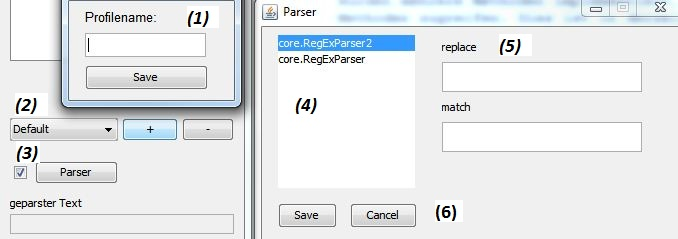
\includegraphics[width=\dimexpr\textwidth]{GUI_profil_parser.png}
  \caption[GUI Beschreibung]%
  {Detailansicht verschiedener GUI-Elemente}
\end{figure}
\begin{enumerate}
\item Profilerstellung, hier kann der Name für ein neues Profil eingegeben werden.
 Hierbei wird ein neues Profil-Objekt mit dem gewünschten Namen erzeugt.
\newpage
\item Profil Kontrollleiste. 
\begin{itemize}
\item Ein DropDown Menü (JComboBox) mit allen verfügbaren Profilen.
\item{[+] - öffnet ein Fenster zur Profilerstellung.}
\item{[-] - löscht das ausgewählte Profil.}
\end{itemize}

\item Parser-Kontrollleiste. 
\begin{itemize} 
\item Checkbox (JCheckBox), (de-)aktiviert das Profil.
\item Parser-Button (JButton), öffnet das Parser-Fenster.
\end{itemize}

\item Parser-Liste (JList), zeigt alle verfügbaren Parser an. Die Parser die
ausgewählt sind werden als aktiv gesetzt beim speichern.

\item Optionaler Bereich, hier können Parser eingestellt werden (bleibt Leer, wenn
ein Parser keine Parameter beinhaltet).
 Dabei werden die Parameter eines Parsers untersucht. String-Parameter bekommen
jeweils ein Label und ein Textfeld zur Eingabe.

\item Buttons, um die getätigten Einstellungen zu speichern / verwerfen. Um dieses
Verhalten zu ermöglichen wird bei Erstellung des Fensters eine Kopie der
aktuellen Einstellungen angelegt.
\end{enumerate}

\section{Parser}
Die Klassen die das Parser-Interface benutzen, dienen der Veränderung der
Einträge.

Die Grundfunktion, also die Manipulation des Eintrags, soll in der Methode
'parse' geschehen. Diese bekommt den Inhalt über ein String Parameter. 

Als Beispiel wurde ein RegEx-Parser umgesetzt. Dieser verändert die Einträge mit
Hilfe eines regulären Ausdrucks. Ein Beispiel um die Funktionalität zu
erläutern: 

RegEx-Parameter:\\
match=\textquotedblleft [\textasciicircum \textbackslash
s]\textquotedblleft  \, (ein Zeichen, außer Leerzeile / -zeichen)a\\
replace=\textquotedblleft  ?\textquotedblleft 

Da String.replaceAll verwendet wird, würde der Parser alle Buchstaben durch ein
Fragezeichen ersetzen. Die Parameter 'match' und 'replace' können entsprechend
über die GUI gesetzt werden. 

Unser Parser benötigt also eigene Parameter. Da dieser Fall öfters auftreten
kann, haben wir uns entschieden, die Parameter bei dem Parser selbst zu
behandeln. Um dieses Ziel in Java zu erreichen bekamen diese intern den Datentyp
'Object'. In unserem Programm wurden nur String-Parameter benötigt, deshalb ist
bei der Dynamisierung nur dieser Fall behandelt. Durch das Abfragen der Klasse
des instantiierten Objektes, ist eine sichere Typisierung weiterhin
gewährleistet. Für Strings bietet sich ein Eingabefeld an, bei boolean Parameter
könnte man z.B. eine Checkbox verwenden. Die Parameter werden in einer HashMap
gespeichert, dementsprechend gibt es für alle Parameter ein gemeinsamen Setter
und Getter.

Bei einem Parse-Aufruf können natürlich auch Fehler auftreten, aber hier ist der
Parser selbst dafür verantwortlich diese abzufangen.

Durch die Plugin-Architektur ist zu der Zeit der Kompilierung nicht bekannt,
welche Parser-Klassen verfügbar sind. Aus diesem Grund ist es notwendig, dass
das Objekt selbst weitere Instanzen erzeugen kann, dies passiert in der
getParser-Methode.

Um die einzelnen Parser in der GUI anzuzeigen, wird zusätzlich ein Name
benötigt. Standardmäßig wird hierfür das Paket verwendet in dem sich der
entsprechende Parser befindet. Angedacht war auch eine Beschreibung, diese wird
allerdings in der Oberfläche nicht angezeigt.

Dank der Plugin-Architektur kann ein Java Entwickler leicht eigene Parser
entwickeln. Hierzu muss das Plugin- und das Parser-Interface implementiert
werden. Es stehen keine Adapter-Klassen bereit, allerdings kann großteil der
Methoden vom RegEx-Parser übernommen werden. Die Methoden parse, getParser und
der Konstruktor müssen den Zweck entsprechend angepasst werden.  

\section{Profile}
Ein Profil verwaltet alle verfügbaren/aktiven Parser. Hierfür wurden mehrere
Methoden implementiert, die auf die Parser-Methoden zugreifen. Dies ist in
derzeitigen Programmstadium nicht notwendig, macht die Wartung allerdings
einfacher. So muss bei einer Zugriffsänderung nur das Profil angepasst werden.

Um die unterschiedlichen Profile auseinander halten zu können, benötigen diese,
so wie die Parser, einen Namen der über die GUI gesetzt werden kann.

In der Methode initParser werden die Parser-Objekte erzeugt. Da der
Plugin-Loader selbst keine Objekte zurück gibt, wird versucht über die getParser
Methode eine Instanz zu erzeugen. Wenn dies fehlschlägt, kann es sich auch um
keinen validen Parser handeln.

\section{Pluginsystem}
Das Pluginsystem besteht aus einem Interface und einem Loader.
Der Loader übernimmt die Aufgaben um ein Plugin zu laden.
Zu diesen Aufgaben gehört es zum Beispiel das Plugin-Verzeichnis zu durchsuchen
und die Plugins zu verifizieren. Danach werden die vordefinierten Methoden der
geladenen Plugins aufgerufen. Um sicherzustellen, dass bei größeren Plugins die
richtige Startklasse verwendet wird muss in der RSF-Datei die Startklasse
angegeben sein.
Bei falscher Startklasse ignoriert der Loader das Plugin.
Die Plugins können auch wärend der Laufzeit nachgeladen werden mit der Reload
Methode. Dabei werden alle vorhanden Plugins verworfen und das
Pluginsverzeichnis wird neu eingelesen und verifiziert.

Das Interface gibt die Methoden für die Plugins vor und definiert so drei
Standardmethoden.  Zu diesen Methoden gehören die Loadmethode, die Startmerthode
und die Stopmethode. 

Die Loadmethode wird beim Laden des Plugins ausgeführt, dabei kann man dem
Plugin den Loader bekannt machen. In der Loadmethode werden auch alle benötigten
Variablen deklariert. Die Startmethode wird nach der Loadmethode aufgerufen und
beinhaltet den eigentlichen Code der ausgeführt werden soll.
Als Finalizemethode kann die Stopmethode angesehen werden. Diese Methode wird
beim Beenden des Plugins aufgerufen.

\begin{figure}[hb]
  \centering
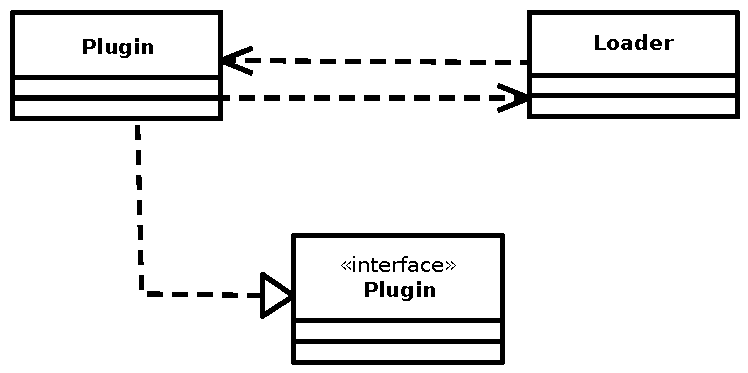
\includegraphics[width=\dimexpr\textwidth]{pluginsystem.pdf}
  \caption[GUI Beschreibung]%
  {
Diese vereinfachte Grafik zeigt den Aufbau des Pluginsystems. >>>>> 
}
\end{figure}

Die Plugin-Pakete sind Jar-Archive mit einer RSF-Datei.
Die RSF-Datei ist nur eine Textdatei mit einer Zeile die den Namen der
Startklasse enthält.

\begin{figure}
  \centering
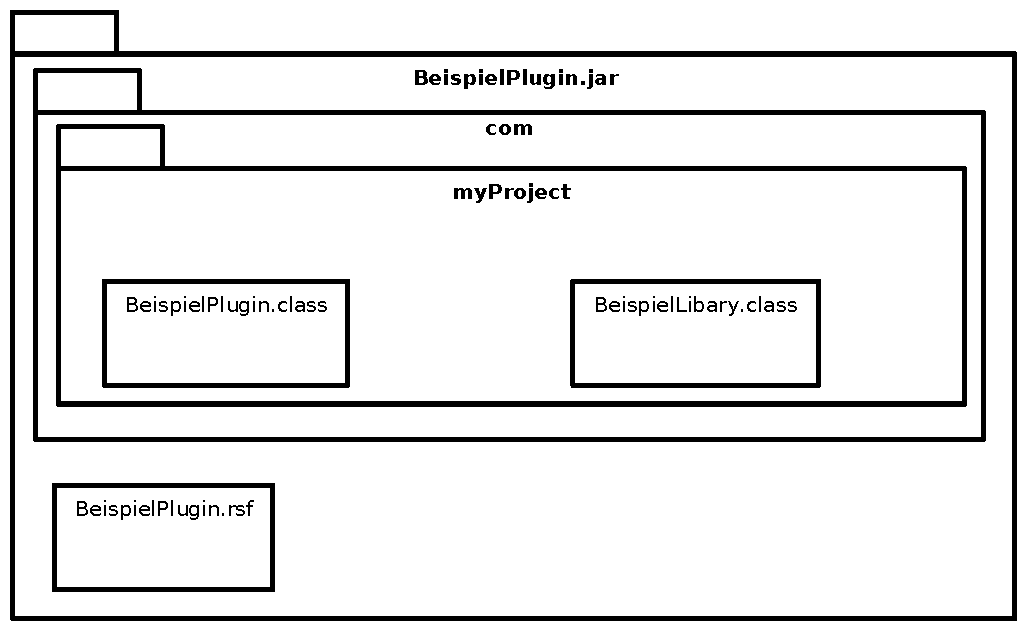
\includegraphics[width=\dimexpr\textwidth]{beispieljar.pdf}
  \caption[GUI Beschreibung]%
  {
Beispiel Aufbau der Jar-Datei.
}
\end{figure}

In diesem Beispiel gibt es das Plugin BeispielPlugin.
Die Jar enthält im Root die RSF Datei. In der RSF steht bei diesem Beispiel
'"com.myProject.BeispielPlugin'`.
Die Jar-Datei kann auch mehrere Klassen Dateien enthalten und dann von der Start
Klasse verwendet werden.

Der Loader hat noch die Invokemethode mit der man eine Methode in einem anderen
Plugin direkt aufrufen kann.

\section{Implementierungsdetails}
Da unsere Implementierung sehr technisch geprägt ist und einige Besonderheiten
enthält wollen wir im folgenden auf genau diese Aspekte eingehen.

\subsection{Clipboard observieren}
Wie bereits in der Darstellung zur OOD zu sehen binden wir das Clipboard in
einem eigenen Objekt ein. Dieses wird von dem Managerobjekt observiert. Das
heißt, dass das Clipboard von der abstrakten Javaklasse Observable erben muss.
Dadurch erbt das Objekt alle nötigen Methoden und Variablen um Überwacht werden
zu können. 

Um ein neues Beobachterobjekt hinzufügen zu können wird die Methode
\texttt{addObserver(obs: Observer)} genutzt. Mit ihrer Hilfe wird das Objekt in
die Liste \texttt{observers} aufgenommen und kann somit informiert werden, wenn
es zu Ereignissen kommt. 

Wenn ein Ereignis eintritt, worüber alle Beobachterobjekte informiert werden
sollen, wird die Methode \texttt{notifyObservers()} aufgerufen. Diese informiert
automatisch alle Beobachter, welche in der Liste \texttt{observers} stehen.

Damit der Manager wiederum das Clipboard überwachen kann muss er das Interface
Observer implementieren. Dieses Interface kennt nur die Methode
\texttt{update(observable: Observable)}, welche in der Klasse Manager
entsprechend mit einer konkreten Funktionalität versorgt wird und dafür sorgt,
dass der neue Eintrag gespeichert und geparsed wird.

Diese lose Bindung des Managers an das Clipboard ist notwendig, da das Clipboard
unbedingt in einem eigenen Thread laufen muss. Der Grund hierfür ist die
einfache Implementierung des Clipboards in Java, denn Java kann nur das
Clipboard auslesen oder neu befüllen, aber es kann nicht ohne weiteren Aufwand
und eine Betriebssysteme spezifische Spezielisierung auf sogenannte
Betriebssystemhooks horchen, die gesendet werden, wenn das Clipboard neu
beschrieben wird. Darum läuft in diesem separaten Thread eine Endlosschleife,
welche regelmäßig das Clipboard ausließt und prüft ob sich der Eintrag geändert
hat.

\subsection{Modulsystem}
Unsere Applikation ist sehr Modular gehalten, das heißt, dass es neben dem
bekannten 3-Schichtenmodell noch auf eine weitere Modularisierung aufbaut.
Das hat den großen Vorteil, dass wir einzelne Komponenten austauschen können,
ohne an der Gesamtfunktionalität etwas zu ändern. So haben wir die Bereiche Gui,
Clipboard, Speichervorgang, Parsen in eigene Bereiche ausgelagert. Außerdem
haben wir ein Pluginsystem implementiert, um die Parser komplett unabhängig vom
eigentlichen Programm entwickeln zu können.

\section{Fazit}
Im Großen und Ganzen ist die Implementierung der Software sehr schnell voran
geschritten. Allerdings gab es einige kritische Punkte zu überwinden. Zum einen
war es schwer die Zusammenarbeit gut zu koordinieren. Hierfür haben wir mehrere
Gründe gefunden, welche vor allem das Zusammentragen der Ergebnisse erschwert
haben. Zum Beispiel war die Absprache in der Gruppe in diesem Projekt nicht so
optimal wie im Vorangegangenen, was sich dadurch gezeigt hat, dass es mehrfach
zu inkompatiblen Vorschlägen beziehungsweise zu sogar zu solchen Umsetzungen
kam. Diese haben die Entwicklung merklich behindert und hätten durch eine
klarere Struktur innerhalb der Gruppe vermindert werden können, da so
sichergestellt gewesen wäre, dass die Vorschläge genauer bewertet und so 
frühzeitig Probleme erkannt worden wären.

Außerdem stellte sich der Gruppenarbeit ein weiteres Problem, da wir mit git
eine Versionierungssoftware genutzt haben, die den SSH-Port 22 nutzt, welcher im
Schulnetz leider grundsätzlich gesperrt ist. Alternativ könnte man zwar auf eine
HTTPS-Verbindung auf Port 443 zurückgreifen, allerdings war auch dies im
Schulnetz nicht möglich, da dieser Port zwar frei ist, jedoch kein echter
Handshake zwischen Client und Server stattfindet. Somit kann auch hier keine
sicher Verbindung hergestellt werden. Da diese aber die Grundlage für das
Übertragungsprotokoll von git ist, war ein arbeiten mit der Software in der
Schule nur eingeschränkt möglich.

Aus diesen genannten Problemen schließen wir, dass wir in den folgenden
Projekten mit einer besseren Absprache wesentlich effizienter arbeiten können.

\end{document}
